\chapter{Legoblokdetectie op basis van CAD modellen}
\label{hoofdstuk:3}
In het voorgaande hoofdstuk werd een na\"ieve methode aangebracht om legoblokken te detecteren. Deze methode worstelde echter met verschillende nadelen waardoor het niet mogelijk was om constructies van legoblokken te detecteren die bestond uit meerdere niveau's. Om dit soort constructies wel te kunnen detecteren moeten we op zoek naar een meer generiek algoritme dat op basis van alle geometrische informatie een legoblok kan detecteren (zodanig dat de blok kan gevonden worden in eender welke legoconstructie). Daarom wordt in dit hoofdstuk een algoritme behandeld dat op basis van features, ge\"extraheerd uit CAD modellen, legoblokken kan detecteren in een videoframe.

Eerst schetsen we kort in sectie \ref{sec:inl_hfdst4} het algoritme. Vervolgens bespreken we in sectie \ref{sec:eval_hfdst4} welke evaluatiemethodes verder in dit hoofdstuk worden gebruikt. Verschillende feature types en classificatie methodes voor dit algoritme worden besproken en vergeleken in secties \ref{sec:feat} en \ref{sec:class} respectievelijk. Tenslotte geven we in sectie \ref{sec:besl_hfdst4} aan waarom deze methode niet kan worden gebruikt in een AR spel om legoblokken te detecteren.

\section{Inleiding} \label{sec:inl_hfdst4}
CAD modellen zijn collecties van punten die de geometrie van een 3 dimensionaal object beschrijven, meestal worden ze gebruikt om objecten in een virtuele 3D wereld voor te stellen. Omdat zulk model alle geometrische informatie over een object bevat, kan deze informatie gebruikt worden om een object in een afbeelding te detecteren. Het grote voordeel is dan dat, aangezien dit model alle geometrische informatie bevat, het object in om het even welke pose kan worden gedetecteerd. Dit is de methode die werd aangebracht in \cite{aubry2014seeing}.

Om CAD modellen te kunnen gebruiken voor object detectie moet eerst nuttig informatie uit deze modellen worden gehaald. In een afbeelding is echter slechts een deel van het object te zien (de afbeelding is namelijk 2D),  daarom is het beter eerst afbeeldingen te genereren van de verschillende poses van het object. Hierna kunnen deze afbeeldingen vergeleken worden met de testafbeelding en afhankelijk van een goede score blijkt welke pose het object in de afbeelding heeft.

Om te bepalen waar het object zich in de afbeelding bevindt wordt gebruik gemaakt van window sliding. Hierbij wordt een rechthoekig window geschoven over de afbeelding en op elke plaats worden de pixels in het window vergeleken met de pixels van de verschillende gegenereerde poses van het object. Om daarenboven ook de schaal van het object te bepalen wordt dit meermaals gedaan met een testafbeelding van verschillende groottes (mbv. een gaussiaanse piramide).

Het vergelijken van het window met de verschillende poses wordt gedaan door van beide features te berekenen en dan via een classificatie methode te vergelijken met elkaar. Hiervoor kunnen verschillende soorten features worden gebruikt en om aan te tonen waarom de keuze in het soort feature zo belangrijk is worden verschillende features in dit hoofdstuk vergeleken met elkaar. Verder worden ook twee verschillende classificatie methodes met elkaar vergeleken.

\section{Evaluatiemethode} \label{sec:eval_hfdst4}
De evaluatie van de verschillende features gebeurt door eerst een classifier te trainen voor alle features en vervolgens de geleerde classifiers te gebruiken voor detectie. 

\begin{table}

\parbox{.45\linewidth}{
	\centering
  	\begin{tabular}{@{}ll@{}} \toprule
    %\cmidrule(r){2-2}
    Parameter & Waarde\\ \midrule
    \textbf{Training} & \\ 
    \# classif. in cascade & 20 \\
    Min. hit rate & 0.999 \\
    Max. false alarm rate & 0.5 \\
    Mode (Haar-like) & ALL \\ \midrule
    \textbf{Detectie} & \\ %\cmidrule(r){2-2}
%    Parameter & Waarde\\ \midrule
    Schaalfactor & 1.1 \\
    Min. \# buren & 15 \\
    Min. grootte & 10x10 (px) \\
    Max. grootte & 100x100 (px) \\ \bottomrule
  \end{tabular}
  \caption{Parameters gebruikt tijdens training en detectie van features met cascade classificatie.}
  \label{tab:param_ccla}
}
\hfill
\parbox{.45\linewidth}{
	\centering
  	\begin{tabular}{@{}ll@{}} \toprule
    %\cmidrule(r){2-2}
    Parameter & Waarde\\ \midrule
    \textbf{Training} & \\ 
    Padding (HOG) & 0x0 (px) \\
    Wind. stride (HOG) & 8x8 (px) \\
    Wind. size (HOG) & 64x64 (px) \\ \midrule
    \textbf{Detectie} & \\ %\cmidrule(r){2-2}
%    Parameter & Waarde\\ \midrule
	Schaalfactor & 1.1 \\
	Hit threshold & 0.4 \\
    Padding (HOG) & 0x0 (px) \\
    Wind. stride (HOG) & 8x8 (px) \\
    Wind. size (HOG) & 64x64 (px) \\ \bottomrule
  \end{tabular}
  \caption{Parameters gebruikt tijdens training en detectie van features met SVM.}
  \label{tab:param_svm}
}
\end{table}

Voor de \textbf{training} werden een 3000-tal positieve en 2946 negatieve samples gebruikt. De positieve samples zijn geconstrueerd door een set van 128 positieve afbeeldingen te transformeren op een willekeurig gekozen negatieve achtergrond (uit de negatieve samples). Deze transformaties helpen om een groter aantal aan positieve samples te genereren en om het effect van belichting en rotaties kleiner te maken. De set van 128 positieve afbeeldingen bestaat uit verschillende zichtpunten op een CAD model van een 2x2 legoblok en enkele foto's van zulke legoblok, allemaal op een witte achtergrond. De zichtpunten zijn gegenereerd van slechts een kwart van de legoblok omdat de legoblok symmetrisch is. De foto's helpen de invloed van belichting op de classifier te minimaliseren aangezien ze werden getrokken in een meer realistische belichting. De parameters die tijdens de training werden gebruikt zijn aangegeven in tabellen \ref{tab:param_ccla} en \ref{tab:param_svm}.

De features werden steeds getraind door een cascade classifier te modelleren (zie sectie \ref{sec:class_ccla}), dit om geen invloed op de resultaten te krijgen door een andere keuze in classificatie methode. Bij de vergelijking tussen de classificatie methodes werd steevast voor de HOG features gekozen om dezelfde reden (zie sectie \ref{sec:feat_hog}).

De \textbf{detectie} gebeurt op twaalf afbeeldingen van een legoblok in verschillende poses. Dit geeft een idee over hoe robuust de features  en classificatie methodes zijn tegen wijzigingen in pose. De parameters die gebruikt werden tijdens de detectie zijn ook aangegeven in tabellen \ref{tab:param_ccla} en \ref{tab:param_svm}.

Bij het vergelijken van features zal eerst naar performantie en robuustheid worden gekeken. Vervolgens wordt aangetoond wat de invloed is van de schaalparameter op de detectie van een legoblok. De vergelijking tussen classificatie methodes focust zich eerst ook op performantie en robuustheid, vervolgens wordt de impact van de \textit{hit threshold} parameter (enkel voor SVM, zie sectie \ref{sec:class_svm}) bekeken. Voor de experimenten die focussen op performantie werd de detectie 10x uitgevoerd op alle twaalf testafbeeldingen. Omdat de training vaak een heel stuk meer tijd vraagt werd deze telkens maar \'e\'en maal uitgevoerd om toch een groffe indicatie te geven van hoe lang zo een training duurt.

De experimenten werden uitgevoerd op een \textbf{machine} met een Intel Core 2 Duo 2,4 GHz processor, een NVIDIA GeForce 320M 256 MB grafische kaart, 8 Gb RAM en Mac OS X 10.10.2. Alle implementaties maken gebruik van OpenCV 2.4.9 (zowel training als detectie) en implementaties met SVM maken gebruik van SVMlight~\cite{joachims1999svmlight}.

\section{Features} \label{sec:feat}

In deze sectie worden drie verschillende soorten features besproken en met elkaar vergeleken: Haar-like~\cite{viola2001rapid}, Multiscale Block Local Binary Patterns~\cite{liao2007learning} (MB-LBP) en Histogram of Oriented Gradients~\cite{dalal2005histograms} (HOG). Tenslotte wordt ook een parts-based feature besproken (gebaseerd op HOG), dat gebruikt werd in \cite{aubry2014seeing}, en waarom deze niet is opgenomen in de vergelijking~\cite{felzenszwalb2010object}.


%In het geval van HOG worden ook twee verschillende methodes voor classificatie met elkaar vergeleken: . Ten slotte wordt kort nog een laatste methode besproken die deels gebaseerd is op HOG~\cite{felzenszwalb2010object}, deze methode zal echter niet worden vergeleken met de andere omdat reeds meermaals werd aangetoond dat deze een te lage performantie heeft om in realtime te gebruiken voor AR.

\subsection{Haar-like} \label{sec:feat_haarlike}
%lienhart2002extended

\begin{figure}
  \centering
  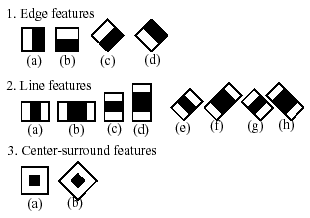
\includegraphics[width=.7\linewidth]{img/haar2}
  \caption{Uitgebreide Haar-like featureset. Het verschil wordt bepaald door de som te nemen van pixels in de witte regio's en af te trekken van de som van pixels in de zwarte regio's.}
  \label{fig:haarUitg}
\end{figure}

Bij de berekening van een Haar-like feature vector wordt het verschil genomen van de som van pixels tussen verschillende rechthoekige regio's. Oorspronkelijk werden vier soorten features gebruikt: twee die elk bestonden uit twee rechthoekige gebieden, \'e\'en soort met drie rechthoekige gebieden en \'e\'en soort met vier rechthoekige gebieden~\cite{viola2001rapid}. Later werden extra features toegevoegd tot de uiteindelijke featureset bestond uit 14 soorten features~\cite{lienhart2002extended}, zie figuur \ref{fig:haarUitg}.

Om goede features te vinden wordt eerst een enorme hoeveelheid aan features aangemaakt. Aangezien dit aantal features een heel stuk hoger is dan het aantal pixels in het window moet een effici\"ente methode gebruikt worden om de juiste features te selecteren. Hiervoor wordt AdaBoost gebruikt, een methode die origineel wordt gebruikt om een classifier sterker te maken. AdaBoost selecteert telkens die feature die de positieve en negatieve samples scheidt zodanig dat de fout zo klein mogelijk is~\cite{viola2001rapid}. Dit impliceert dat elke feature ook een threshold bevat die aangeeft wanneer deze feature een detectiewindow juist of onjuist classificeert. De uiteindelijke feature vector van het volledige detectiewindow is de set van de geselecteerde features.

%\paragraph{Voordelen}
%\begin{itemize}
%	\item Eenvoudig te berekenen;
%	\item Snelle detectie met behulp van CCLA.
%\end{itemize}
%
%\paragraph{Nadelen}
%\begin{itemize}
%	\item Duurt lang om te trainen;
%	\item Performantie bij detectie hangt af van aantal features voor elke classifier in de cascade;
%	\item Kan niet tegen occlusie, omdat dit de waarden van pixels sterk veranderd en dus ook de feature vector.
%\end{itemize}

\subsection{MB-LBP} \label{sec:feat_mblbp}

\begin{figure}
  \centering
  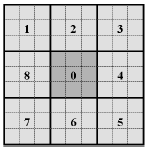
\includegraphics[width=.3\linewidth]{img/lbp}
  \caption{Een 9x9 MB-LBP operator: elk blok bestaat uit 9 pixels.}
  \label{fig:lbp}
\end{figure}

Een MB-LBP feature is een uitbreiding op de originele LBP feature waarin elke pixel werd vergeleken met zijn acht buren. Deze acht buren werden steevast in dezelfde volgorde overlopen en telkens een buur een grotere intensiteit had dan de pixel zelf werd een '1' genoteerd, in de andere gevallen een '0'. Zo wordt voor elke pixel een getal verkregen van acht bits dat de gradi\"ent van de pixel voorstelt in de verschillende pixels~\cite{ojala1996comparative}.

Hier wordt de MB-LBP feature gebruikt in plaats van de oorspronkelijke LBP omdat deze meer robuust is. In de MB-LBP variant worden, in plaats van een pixel met zijn buren te vergelijken, blokken van pixels met hun buren vergeleken (zie figuur \ref{fig:lbp}). Hierdoor wordt is de feature meer robuust en encodeert het bovendien, naast microstructuren, ook macrostructuren in een afbeelding~\cite{liao2007learning}. 

Om de feature vector van een volledig window te berekenen wordt het window in cellen opgesplitst en vervolgens histogrammen van de MB-LBP features binnen een cel. De histogrammen van elke cel worden ten slotte geconcateneerd om de feature vector te bekomen.

%\paragraph{Voordelen}
%\begin{itemize}
%	\item Eenvoudig te berekenen;
%	\item Kan snel worden getraind;
%	\item Snelle detectie met behulp van CCLA.
%\end{itemize}
%
%\paragraph{Nadelen}
%\begin{itemize}
%	\item Performantie bij detectie hangt af van aantal features voor elke classifier in de cascade;
%	\item Kan niet tegen occlusie, omdat dit de waarden van pixels sterk veranderd en dus ook de feature vector.
%\end{itemize}

\subsection{HOG} \label{sec:feat_hog}

Bij een HOG feature worden eerst gradi\"enten van alle pixels in een window berekend. Vervolgens wordt het window onderverdeeld in cellen en wordt voor elke cel een histogram van de gradi\"enten gemaakt. Om problemen met belichting en contrast te voorkomen worden cellen gecombineerd tot blokken waarover deze histogrammen worden genormaliseerd. Ten slotte worden alle histogrammen geconcateneerd (net als bij MB-LBP) om een feature vector van het window te bekomen~\cite{dalal2005histograms}.

%\paragraph{Voordelen}
%\begin{itemize}
%	\item Onafhankelijk van belichting en contrast: kijkt vooral naar geometrie van een object;
%	\item Kan snel worden getraind;
%	\item Snelle detectie met behulp van CCLA of SVM.
%\end{itemize}
%
%\paragraph{Nadelen}
%\begin{itemize}
%	\item Detectie is trager dan bij Haar-like of LBP features;
%	\item Kan niet tegen occlusie, omdat dit de gradi\"enten van een afbeelding sterk wijzigt en dus ook de feature vector.
%\end{itemize} 

\subsection{Deformed parts-based} \label{sec:feat_part}
Deformed parts-based modellen is een type feature dat bestaat uit twee onderdelen: een HOG feature van de volledige window (root filter) en aantal kleinere HOG features van een subwindow (part filters). Deze verschillende part filters worden gedefinieerd door een anker punt ten opzichte van de plaats van de root filter en een functie die alle mogelijke plaatsen van deze part filter beschrijft relatief ten opzichte van het anker punt. De score van de hypothese dat een window het te detecteren object bevat wordt berekend door de sommatie te nemen van het verschil tussen de score van de filter (HOG feature) en een kost voor de vervorming van de filter. Dit model maakt het HOG feature een stuk meer flexibel voor vervormingen of andere poses van een object ~\cite{felzenszwalb2010object}.

Een groot nadeel van deze methode is dat ze nogal wat rekenwerk vraagt om uit te voeren en dus ongeschikt is voor gebruik in AR. Dit is zelfs eerder aangetoond in andere state-of-the-art papers die de performantie hebben kunnen verhogen. Hoewel bijvoorbeeld in paper \cite{yan2014fastest} wordt aangegeven dat 40 FPS haalbaar is, is dit slechts na parallellisatie en bovendien op een desktop computer. Zulke resultaten zullen dus (voorlopig) niet gehaald kunnen worden op een mobiel apparaat om te gebruiken voor AR. Wegens tijdsbeperkingen hebben we dit niet aangetoond.

\subsection{Vergelijking}
In deze sectie worden de eerste drie besproken feature-types met elkaar vergeleken. Ze worden eerst vergeleken qua performantie en robuustheid. Tenslotte wordt onderzocht wat de impact is op de performantie en robuustheid bij het wijzigen van de schaalfactor.

%\paragraph{Eigenschappen}

%\begin{table}
%  \centering
%  \begin{tabular}{@{}lccc@{}} \toprule
%    & \multicolumn{3}{c}{Features} \\ \cmidrule(r){2-4}
%    & Haar-like & MB-LBP & HOG\\ \midrule
%    Berekening & Snel & Snel & Traag \\
%    Occlusie & Neen & Neen & Neen \\
%    Scope & Lokaal & Globaal & Globaal \\\bottomrule
%  \end{tabular}
%  \caption{Feature eigenschappen.}
%  \label{tab:feat_eig}
%\end{table}
%
%In tabel \ref{tab:feat_eig} worden een aantal eigenschappen opgesomd, waarin de verschillende soorten features met elkaar worden vergeleken. 
%
%De berekening van Haar-like en MB-LBP features is snel, omdat dit kan door gebruik te maken van integraal afbeeldingen~\cite{viola2001rapid}. HOG is ten opzichte van Haar-like en MB-LBP features echter 
%
%Zowel bij Haar-like als bij MB-LBP features kan AdaBoost gebruikt worden om een krachtige classifier te construeren.

\paragraph{Performantie}

De vergelijking van performantie tussen verschillende soorten features bestaat uit twee onderdelen: enerzijds de snelheid bij training van de classifier en anderzijds de snelheid bij detectie. 

Tabel \ref{tab:feat_perf} toont dat een classifier op basis van HOG features sneller kan worden getraind dan een classifier op basis van LBP features en dat deze laatste sneller kan worden getraind dan een classifier op basis van Haar-like features. We merken vooral op dat er een groot verschil is tussen de tijd nodig om een HOG classifier te trainen en tijd nodig om een LBP of Haar-like classifier te trainen. Dit valt als volgt te verklaren: bij het trainen van een Haar-like classifier wordt eerst voor elke window een enorme hoeveelheid aan features gegenereerd die vervolgens wordt uitgeselecteerd met AdaBoost~\cite{freund1995desicion}. Deze hoeveelheid aan features is vele malen groter dan het aantal pixels in het window, in tegenstelling tot MB-LBP en HOG waarbij voor elk window enkel een histogram wordt opgesteld (in feite worden voor MB-LBP meerdere histogrammen geconcateneerd).

Uit de snelheid in detectie kunnen we vooral opmerken dat de detectie van MB-LBP een stuk sneller gaat dan detectie van Haar-like en HOG. De reden hiervoor is simpelweg dat bij MB-LBP gewoon integer waarden worden vergeleken terwijl bij Haar-like en HOG features floating point getallen moeten worden vergeleken. 

\begin{table}
  \centering
  \begin{tabular}{@{}lcc@{}} \toprule
    & \multicolumn{2}{c}{Gemiddelde performantie} \\ \cmidrule(r){2-3}
    Feature & Training & Detectie (ms)\\ \midrule
    Haar-like & > 2 dagen & TODO \\
    MB-LBP & TODO & 43.71 \\
    HOG & TODO & 189.36 \\ \bottomrule
  \end{tabular}
  \caption{Feature performantie.}
  \label{tab:feat_perf}
\end{table}

\paragraph{Robuustheid}

Uit de resultaten van figuur \ref{fig:featRobuust} kan worden afgeleid dat detectie met behulp van HOG, getraind via een SVM de beste resultaten geeft: slechts op \'e\'en afbeelding uit de testset was een vals positief resultaat aanwezig en op 2 afbeeldingen uit de testset na werd de legoblok correct gevonden door de classifier.

Figuur \ref{fig:featRobuust} toont dat de HOG features erg slechte resultaten vertoont: slechts 4/12 keer wordt de legoblok werkelijk gevonden in de frame.

\begin{figure}
  \centering
  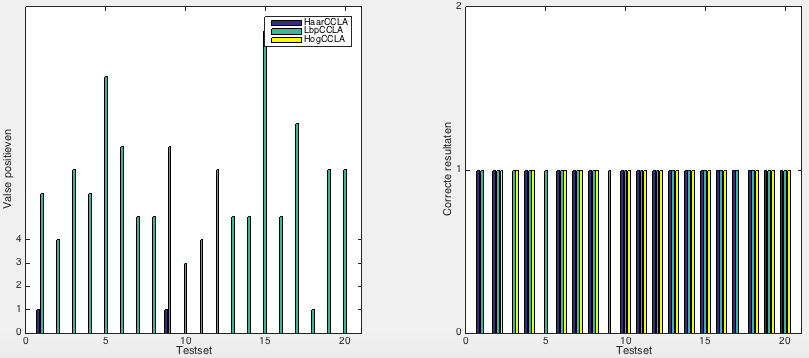
\includegraphics[width=\linewidth]{img/FeatRobust}
  \caption{Feature robuustheid.}
  \label{fig:featRobuust}
\end{figure}

\section{Classificatie methodes} \label{sec:class}
In deze sectie worden de volgende classificatie methodes besproken: Cascade Classifiers \cite{viola2001rapid} (CCLA) en Support Vector Machines~\cite{joachims1999svmlight} (SVM). Vervolgens worden beide methodes vergeleken op vlak van robuustheid en performantie. Ten slotte wordt de impact bekeken van de \textit{scale factor} parameter op robuustheid en performantie CCLA en hetzelfde wordt gedaan met de \textit{hit threshold} parameter voor SVM.

\subsection{CCLA} \label{sec:class_ccla}
Bij een \textbf{CCLA} wordt een classifier getraind door een aantal feature classifiers te combineren. Elk van deze classifiers bestaat uit een aantal features op basis waarvan elke subwindow van een frame wordt geclassificeerd. Zulke cascade classifier werkt door eerst elke subwindow van de frame te laten evalueren door de eerste classifier, indien de eerste classifier de subwindow aanvaardt triggert dit een evaluatie door de volgende classifier in de cascade. Enkel wanneer een window door alle classifiers is aanvaard, kan er vanuit worden gegaan dat dit window het te detecteren object bevat. Door een cascade van classifiers te gebruiken moet elke classifier van de cascade niet al te sterk zijn waardoor negatieve windows al sneller kunnen worden afgevoerd, wat de detectie des te sneller maakt.

\subsection{SVM} \label{sec:class_svm}
Een \textbf{SVM} classificeert op een andere manier: elk subwindow wordt voorgesteld als een p-dimensionele vector in een p-dimensionele ruimte. Met behulp van (p-1)-dimensionele hyperplane worden de subwindows gesplitst in twee groepen: de ene groep wordt aanvaard, de andere niet. Deze lineaire classifier was het oorspronkelijke algoritme~\cite{vapnik1963pattern}, later werd ook een methode ontwikkelt voor non-lineaire classificatie~\cite{boser1992training}.

\subsection{Vergelijking}

\paragraph{Robuustheid}

Figuur \ref{fig:classRobuust} toont de robuustheid van de twee classifier methodes. Merk op dat de grafiek met valse positieven is weggelaten omdat deze in beide gevallen overal nul was. Er is duidelijk weinig verschil tussen de twee methodes qua robuustheid:  de SVM methode detecteert \'e\'en legoblokje meer.

\begin{figure}
  \centering
  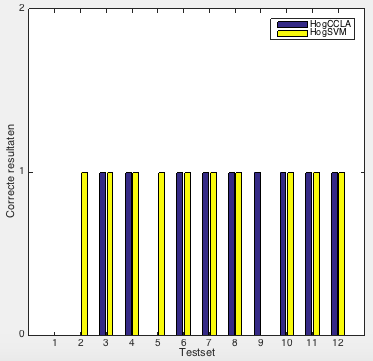
\includegraphics[width=0.5\linewidth]{img/ClassRobust}
  \caption{Robuustheid classifier methodes.}
  \label{fig:classRobuust}
\end{figure}

\paragraph{Performantie}

Tabel \ref{tab:class_perf} toont een vergelijking van de performantie tijdens de training en de detectie. Dit toont aan dat de snelheid van CCLA hoger ligt bij detectie maar niet bij training. Dat de detectie langer duurt bij een SVM is logisch aangezien het een lineaire classifier is (geen cascade die de snelheid verhoogt). De training snelheid ligt lager bij een SVM omdat deze geen cascade moet opstellen, terwijl CCLA dit wel moet doen.

\begin{table}
  \centering
  \begin{tabular}{@{}lcc@{}} \toprule
    & \multicolumn{2}{c}{Gemiddelde performantie} \\ \cmidrule(r){2-3}
    Feature & Training & Detectie (ms)\\ \midrule
    CCLA & TODO & 189.36 \\
    SVM & 1m55s & 244.94 \\ \bottomrule
  \end{tabular}
  \caption{Performantie classifier methodes.}
  \label{tab:class_perf}
\end{table}

\paragraph{Schaalfactor}

De schaalfactor is een parameter die bepaalt hoe sterk de schaal van het window wordt gewijzigd tussen een minimum en maximum grootte. Dus wanneer deze kleiner wordt zullen normaal gezien meer iteraties nodig zijn, terwijl een nauwkeurigere detectie plaatsvindt.

Om de impact van de schaalfactor te bepalen, wordt de performantie en robuustheid van de HOG feature vergeleken wanneer de schaalfactor 1.01, 1.05, 1.10, 1.15, 1.20 en 1.25 bedraagt. Uit figuur \ref{fig:featScale} is het duidelijk dat aan de verwachtingen voldaan is: de performantie is hoger (het aantal ms daalt) bij een hogere schaalfactor, terwijl het aantal correcte detecties daalt. Het aantal valse positieven werd ook gemeten maar deze was 1 bij schaalfactor 1.01 en 0 voor de rest.

Opmerkelijk is echter dat het aantal correcte poses hoger ligt bij SVM dan bij CCLA. Maar hoewel de detectie beter is laat de performantie echter te wensen over. De oorzaken hiervoor kunnen als volgt verklaard worden: Een SVM is een lineaire classifier die vergeleken kan worden met \'e\'en enkele classifier uit een cascade. Om een voldoende goede detectie te behalen moet een SVM dus erg correct kunnen classificeren, dit vergt meer tijd aangezien een cascade juist is ontwikkeld om effici\"enter te zijn dan een enkele classifier. Aangezien de SVM een hogere robuustheid haalt is het dan ook logisch dat de performantie hoger is.

\begin{figure}
  \centering
  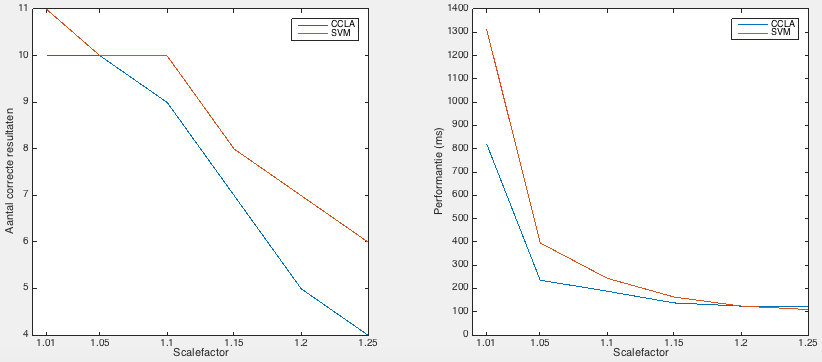
\includegraphics[width=\linewidth]{img/scaleFact}
  \caption{Impact schaalfactor op performantie en robuustheid van HOG feature.}
  \label{fig:featScale}
\end{figure}


%Om deze soorten features met elkaar te vergelijken werden afbeeldingen van één legoblok uit verschillende zichtpunten genomen. Vervolgens werd een classifier getraind voor elke soort feature. Bij de detectie werd nagegaan hoeveel false positives en hoeveel correcte detecties werden gedaan (aangezien slechts 1 legoblok werd gebruikt is het maximum aantal detecties altijd 1).


%\subsection{Een item}
%De bijbehorende tekst. Denk eraan om de paragrafen lang genoeg te maken en
%de zinnen niet te lang.
%
%Een paragraaf omvat een gedachtengang en bevat dus steeds een paar zinnen.
%Een paragraaf die maar \'e\'en lijn lang is, is dus uit den boze.

\section{Discussie / Besluit} \label{sec:besl_hfdst4}

\begin{figure}
  \centering
  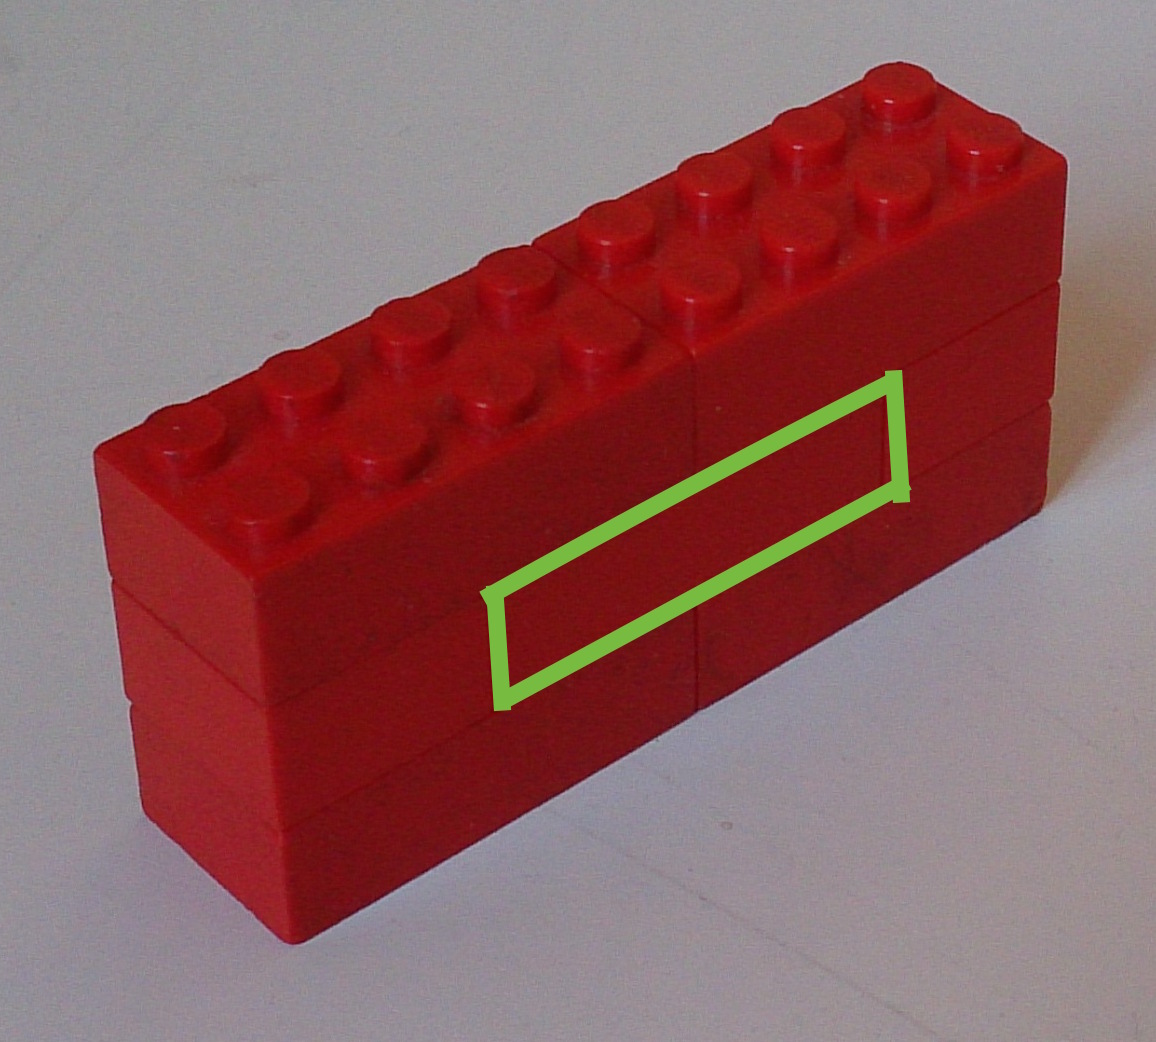
\includegraphics[width=0.5\linewidth]{img/brickWall}
  \caption{Een voorbeeld van een legoblokconstructie waarin het groen omlijnde vlak het enige is wat we van die legoblok zien.}
  \label{fig:brickWall}
\end{figure}

In dit hoofdstuk werd onderzocht welke feature types en classifier methodes beter werken voor detectie van legoblokken. Zo is aangetoond dat HOG de meer robuuste feature type is en dat MB-LBP de meest performante van de drie is. Verder werd aangegeven dat een vierde type feature (parts-based deformable modellen) te traag is om nuttig te gebruiken in een AR applicatie. Ten slotte toonde de vergelijking tussen classifier methodes aan dat detectie met een SVM classifier vaak trager is maar tegelijk ook meer robuust. De methode die in dit hoofdstuk werd onderzocht is echter niet nuttig om te gebruiken in een AR spel om legoblokken te detecteren en hier is waarom:

Hoewel het wel mogelijk is om een enkele legoblok te detecteren is het erg moeilijk om in een constructie van legoblokken de blokken afzonderlijk te detecteren. Dit resulteerde telkens in erg slechte resultaten, zelfs wanneer het beste type feature en de beste classificatie methode werd gekozen. Dit wordt hoofdzakelijk veroorzaakt door de enorme hoeveelheid aan occlusie die een legoblok in een constructie grotendeels verbergt. Hierdoor is slechts een erg beperkt deel van de legoblok (in sommige gevallen slechts \'e\'en vlak, zie figuur \ref{fig:brickWall}) zichtbaar wat het erg moeilijk maakt om met features een legoblok te detecteren. Zelfs indien op voorhand een optimale pose zou worden gekozen kan voor sommige legoblokken enkel \'e\'en vlak zichtbaar zijn in de afbeelding.

Deze redenering leidt tot een volgend resultaat: het is erg moeilijk, zo niet onmogelijk, om in een legoconstructie alle legoblokken apart te detecteren. Daarom moeten we proberen om, in plaats van de blokken individueel te proberen detecteren, ze als groter geheel te detecteren. Zulke legoconstructie kunnen we zien als een flexibele legoblok die eender welke hoogte, diepte en breedte kan hebben. Dat is exact waarvoor parts-based deformable modellen voor worden gebruikt maar zoals aangehaald in sectie \ref{sec:feat_part} is deze methode veel te traag om te gebruiken in AR. Dat is de reden waarom in de volgende sectie een sneller alternatief wordt voorgesteld dat wel gebruik maakt van het idee dat lego constructies moeten gedetecteerd worden in plaats van individuele legoblokken. Hierbij wordt echter wel afgestapt van het idee om CAD modellen te gebruiken.

%Er zijn in een hoofdstuk verschillende onderwerpen. We zullen nu
%veronderstellen dat dit het laatste onderwerp is.

%\subsection{Een item}
%Maak ook geen misbruik van opsommingen. Voor korte opsommingen gebruik je
%geen ``\verb|itemize|'' of ``\texttt{enumerate}'' commando's. Doe dus
%\emph{niet} het volgende:
%\begin{quote}
%  De Eiffeltoren bevat drie verdiepingen:
%  \begin{itemize}
%  \item de eerste;
%  \item de tweede;
%  \item de derde.
%  \end{itemize}
%\end{quote}
%Maar doe:
%\begin{quote}
%  De Eiffeltoren bevat drie verdiepingen: de eerste, de tweede en de derde.
%\end{quote}

%\section{Besluit}
%BESLUIT VAN DIT HOOFDSTUK %TODO 
%Als je in dit hoofdstuk tot belangrijke resultaten of besluiten gekomen
%bent, dan is het ook logisch om het hoofdstuk af te ronden met een
%overzicht ervan. Voor hoofdstukken zoals de inleiding en het
%literatuuroverzicht is dit niet strikt nodig.

%%% Local Variables: 
%%% mode: latex
%%% TeX-master: "masterproef"
%%% End: 
